\chapter[SCP-178 “3D”眼镜]{
    SCP-178 "3-D" Specs\\
    SCP-178 “3D”眼镜
}

\label{chap:SCP-178}

\begin{figure}[H]
    \centering
    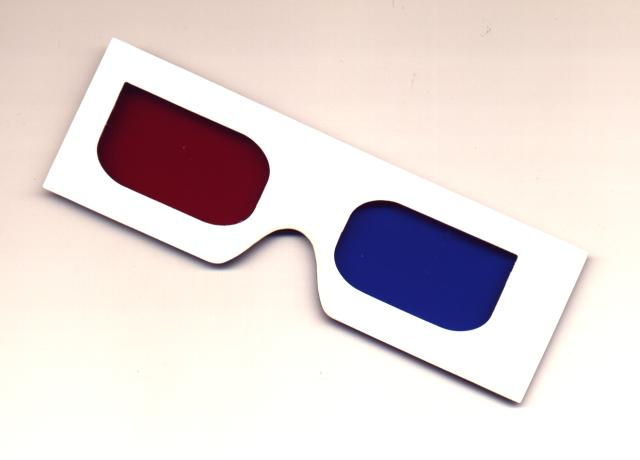
\includegraphics[width=0.5\linewidth]{images/SCP-178.jpg}
    \caption*{镜腿折合的SCP-178。}
\end{figure}

\bb{项目编号:}SCP-178

\bb{项目等级:}Euclid

\bb{特殊收容措施:}在不接受测试时,SCP-178应当被存储在一个由不少于两名武装过的三级人员看守的3级异常物品收容装置内。只有在经过四级及以上的人员的书面许可之后对象才能从容器中被移出。\bb{在事故178-14-Alpha之后,所有试验都必须进行远程监控,并明令禁止除受试者以外的所有人员在试验进行时进入试验区。}

\bb{描述:}SCP-178是一副白色的立体(3D)眼镜,由一个长方形的白色纸板框架和左右分别为蓝色与红色的塑料镜片组成。除了其纸板上符合其年龄的轻微变色以外,该物品具有不寻常的物理特性。当佩戴它时,佩戴者会在正常的环境以外感知到大量的大型两足生物。根据报告显示这些生物表现出善良并偶尔好奇的行为特征(有报告说这种生物靠在工作人员的肩上并好奇地打量他们)。佩戴者\bb{及任何其他人员}(见事故报告178-14-Alpha)与这些生物直接进行接触的企图都会导致参与者突然遭到重创。这一伤害会让佩戴者迅速并持续地走向死亡。创口的外观始终表现为被三个平行的长度在14.2厘米到27.4厘米之间,厚度在2.8厘米到8.1厘米之间的尖锐物体所切割出来的。在测试过程中记录和测量设备没有检测到任何异常状况,包括在测试者受到伤害时。测试者没有听到这些生物发出任何声音。长期暴露于项目中不会有什么影响。透过项目所看到的的图像表现出三维的效果。

\bb{附录1:}项目于19██年██月██日在美国田纳西州的███████由潜伏在美国鱼类和野生生物服务局的特工{[}删除]在去该处调查一起关于一个█岁的儿童被发现死在自家二楼的卧室中,并在死前受过不同寻常的伤害的案件时收容。特工{[}已编辑]在那个孩子被发现的地方看到了一副血淋淋的摩天轮的立体图片,并在一番寻找后在那个孩子的床下发现了该项目,很明显它是在孩子死前的剧烈痛苦中被扔到那里去的。特工{[}已编辑]随即直接把收容小队叫到了他所在的地方。在收容小队到达之后,特工{[}已编辑]戴上了项目然后看了看那张图片并表示没什么异常,直到他向左转过头时,他才发现一个大约“一英寸长”的生物正靠在他的肩膀上看着立体图片。特工{[}已编辑]报告说在房间里还有其他的生物也在观察着他和收容小队。特工{[}已编辑]并未试图与这些生物进行接触,因此这个物品没有发生事故就被收容了。

\bb{附录2:}所有实验都被记录在\hyperref[sec:DOC-scp-178-log]{文件178-E}中。

\bb{附录3:}所有4级人员都必须阅读事故报告178-14-Alpha。阅读事故报告178-14-Alpha是所有四级及以上人员批准对该物品的实验的前提条件。\\
\bb{警告:不遵守附录3将会受到纪律处分。}

\newpage
\section{文件\#178-E}

\label{sec:DOC-scp-178-log}

\ii{\bb{所有与SCP-178的互动的实验都会记录在这里}}\bb{- ██████████博士}

\hr

\bu{实验178-e-1}

\bb{执行者:}██████████博士,由█████博士和███████博士辅助

\bb{实验日期:}██\slash ██\slash 19██

\bb{实验程序}:D级人员安置在内有SCP-178的密封测试室。测试室将会透过防弹玻璃外的邻近的控制室和视听记录设备进行观察。D级人员被要求配带SCP-178和在观察到异常状况时回报。

\bb{实验结果:}对象D-17831(男性,41岁,精神没有异常)被置于测试室内,要求对象带上SCP-178。对象没有被告知SCP-178的异常特性。对象跟随指示,然后立即扔SCP-178,然后感到忧伤并著双眼发出感到恐惧的叫声。研究员命令对象描述令它忧伤的根源。对象没有答复。研究员尝试安抚对象。对象没有掩面,看著四周的时候回应,对象仍感到忧伤。研究员指示对象再一次描述它忧伤的原因。对象回答当他带上SCP-178时,他确他面前有个不能碓定的实体,而且紧贴在面前。研究员指示对象形容该实体的细节。对象形容面前的实体是“丑陋”和“有太多的眼”。研究员指示对象进一步描述该实体的细节。对象声明他在移除SCP-178没有察觉到更多的细节。研究员指示对象再次戴上SCP-178。对象不配合。研究员重复指示。对象仍不配合。研究员以杀死威迫对象合作。对象仍不配合。测试结束,对象被安置以监察长期暴露在SCP-178下的影响。在回复正常行为前两日,对象表现出轻微的妄想症。监察结束,对象在三十日后被处决

\ii{笔记:这次测试看起来不太有用,但至少确定我们确实有异常事物出现}

\hr

\bu{实验178-e-2}

\bb{执行者:}██████████博士,由█████博士和███████博士辅助

\bb{实验日期:}██\slash ██\slash 19██

\bb{实验程序:}D级人员安置在内有SCP-178的密封测试室。测试室将会透过防弹玻璃外的邻近的控制室和视听记录设备进行观察。D级人员被要求配带SCP-178和在观察到异常状况时回报。

\bb{实验结果:}对象D-63164(女性,31岁,精神没有异常)被置于测试室内,要求对象带上SCP-178。对象没有被告知SCP-178的异常特性。对象按要求执行和立即发出咒骂并后退至测室的墙壁,注视著某物一个小时。研究员指示对象去描述他所见的事物。对象把自己的背压到测试室的墙后和说明他看到了一个实体站在测试室的墙之间,并且看著墙。研究员指示对象形容该实体的细节。对象描述该实体是两足,有两个圆锥突出的附属器官和一个光滑的头部。研究员指示对象进一步提供细节。对象开始描述实体,对象突然感到忧虑,并说出“我的天,它正看著我”的言论。对象在测试室内崩溃,仍然凝视著某个方向。研究员查问该实体是否显露敌意。对象说他没有移动,但仍看著它。对象指示移除SCP-178。对象拒绝,并说它并不相信这是实体。对象被告知如果不合作将会被消灭。对象移除SCP-178,并开始忧虑地看著四周,说自己没有看到实体。对象被指示戴著SCP-178。对象服从并说该实体仍看著它。对象被指示去汇报更多实体行为的变化。在2分37秒后,对象说实体没有看著它。对象并说该实体再一次看著墙。对象回报在17分55秒实物没有任何行为的改变。测试结束。

\ii{笔记:实验对象所看到的奇怪事物看起来很奇怪,这东西得到了基金会的注意。我们不能从任何的记录设备得到任何数据。我想知道这个实体是真的存在,或是由这东西产生的幻觉。}

\hr

\bu{实验178-e-3}

\bb{执行者:}██████████博士,由█████博士和███████博士辅助

\bb{实验日期:}██\slash ██\slash 19██

\bb{实验程序:}D级人员将会置于收容SCP-178的安全测试室中。测试室将会靠邻近装有防弹玻璃的控制室和摄影设备进行观察。一幅有著颜色为红色和蓝色的碎片状图像,会挂在测试室的墙上,以及该墙的对面放置一个装有十个标准网球的塑胶篓子。对象将会被告知SCP-178是测试新型“3-D眼镜”,并说明在看著碎片状的图像时,可以看到活动中的3d图象。D级人员将被要求带上SCP-178并汇报观察到的情况,若对象察觉到任何实体出现,他会被指示向其实体抛网球。

\bb{实验结果:}D-51441(男性,27岁,有著纵火、凶杀的记录,精神没有异常)被要求站在有著碎状图案的墙的对面,及配带SCP-178。对象服从要求,表现出惊讶和不舒服。对象指示去形容看到的事物。对象指出他看到两个实体站在房间中,一个(下称实体1)背对对象站在图片旁,另一个(下称实体2)从左向右穿过房间。对象发出设计这个实体的人是心理不平衡的意见。对象被指示去描述实体2的步态,对象指出实体2是用它的腿和上部附属器官去走路。对象模仿实体2的步态,实体2的步态类似大猩猩“是不是某人拼装错他的骨架”。研究员询问两个实体是否相似。对象回应它们的身形有一段距离,但是他们大致相同。然后对象继续描述实体特征,以判断该实体是否和实验\#178-e-2相同。对象被指示用拿一个网球扔向实体2,对象服从命令。研究员和影像设备均观察到小球不间断地移动直到球打中到测试室的另一边。对象表现出惊讶和忧虑,对象尝试离开后0.7秒,他的身体出现严重割伤。在4.7秒后表面的割偒持续出现,直至对象可能因严重出血和心理创伤死亡。死亡的对象被验尸发现伤口一致都是由三个利器挥斩而成,锐器相当的厚并逐渐变窄,大约是长17cm,深4cm。对对象所挥的球进行的分析发现只有少量汗液,汗液是对象D-51441的。

\ii{笔记:我{[}咒骂]!它不喜欢被骚扰。另一方面,球在空气中飞行时,就像没有东西似的,和从那个死尸上我们不能知道球实际上有没有穿过实体。这仍然是还远远不能定论,但是裂伤的类型与该项目所在的站点的发现吻合,至少我们已经出现很多任何疑问,这是很危险的。这是一个很有趣的事。去记录到目前为止的实体都有一致的外貌,尽管测试对象都不一样。我想知道任何的对象和实体之间的非暴力性互动是否可行的。}

\hr

\bu{实验178-e-4}

\bb{执行者:}██████████博士,由█████博士和███████博士辅助

\bb{实验日期:}██\slash ██\slash 19██

\bb{实验程序:}D级人员将会置于收容SCP-178的安全测试室中。测试室将会靠邻近装有防弹玻璃的控制室,摄影设备,红外线照相机,电磁辐射探测器和活动探测器以进行观察。一幅有著颜色为红色和蓝色的碎片状图像,会挂在测试室的墙上。对象将会被告知SCP-178是测试新型“3-D眼镜”,并说明在看著碎片状的图像时,可以看到活动中的3d图象。D级人员将被要求带上SCP-178并汇报观察到的情况,若对象察觉到任何实体出现,他会被指示与实体进行交流。

\bb{实验结果:}D-84291(女性,19岁,精神没有异常)被要求站在有著碎状图案的墙的对面,及配带SCP-178。对象服从要求和立即表达出厌恶感。对象被要求说明她所看见的事物。对象形容该实体与之前所汇报的实体相似,并且离对象大约2米处,并且看著对象。对象被只是去尝试和它说话。对象因他为何要尝试和这个活动实体说话而困惑。研究员重复指示。对象表示不快,然后以沉闷的口气对实体说:“你好,奇怪的东西,你今天好吗?”在说话后的0.2秒裂伤开始出现在对象的躯体和腹部上,对象的右臂手肘在2.4秒后断裂。当裂伤和对象的声音在8.4后停止,对象可能死亡。对死亡对象的医学解剖发现出同样的裂伤,表明了该锐器大约有21cm长,5cm宽。

\ii{笔记:我猜我们能假定和实体尝试任何的互动,最后取决于态度。和任何的探不到任何东西。我们建立了一个模式,但是重要的问题是对象的死亡是否是因为SCP-178还是这些外在实体。我想知道没有配带SCP-178的对象是否可以受到SCP-178的影响。}

\hr

\bu{实验178-e-5}

\bb{执行者:}██████████博士,由█████博士和███████博士辅助

\bb{实验日期:}██\slash ██\slash 19██

\bb{实验程序:}两个D级人员将被置于收容SCP-178的安全测试室中。测试室将会靠邻近装有防弹玻璃的控制室,摄影设备,红外线照相机,电磁辐射探测器和活动探测器以进行观察。两个对象将会被告知SCP-178的所有基本知识。其中一个对象(被称为对象1)将会配戴SCP-178并把任何测试室察觉到的实体的对象的位置和外貌情况描述给另一个对象(被称为对象2)。对象2将会尝试和实体互动。

\bb{实验结果:}对象1(D-61955,女性,35岁,与3宗谋杀案有关,严重的人身伤害,没有心理异常)和对象2(D-61955,女性,27岁,没有心理异常)被置于测试室内。对象1指示配带SCP-178。对象1向研究员表示不赞。对象2同意其想法。研究员提醒对象如果对象不合作将会被处决。对象1配戴SCP-178并开始发出咒骂。对象2表达出忧虑,其原因和对象1出现惊惶失措的原因一样。对象2转身并说出她看不到任何不正常之处。研究员向对象保证所察觉的实体是无害的以令其冷静并指示对象1去协助对象2去与实体交流。对象1说这有一个的实体站在她一英尺面前,而实体比对象2高两英尺。对象2询问实体是否看著她。对象1回应肯定地回。答对象2尝试去冷静自己和继续看著她认为是实体的头所在的地方和说“唔,你好”在对象2的颈部被折断前的0.9秒对象2的躯体和脸开始出现撕伤。对象1忧虑地大叫和跑向测试室大门。对象1尝试和威胁打开大门,但不成功,5秒后转身和大概对所看到的实体说“不!给我滚开!”对象1的腹部和躯干出现裂伤。在17.3秒后,对象1身上的裂伤和发声同时停止。死亡对象的医学解剖出现两种不同种类的裂伤。对象2身上一些有关的裂伤都由三个是由长27cm,至少宽8cm的利器所形成,而对象1身上一些有关的裂伤都由三个是由长14cm,宽3cm的利器所形成。

\ii{笔记:我们仍不知道该实体是否真的存在或者只是SCP-178的幻觉,但是我们知道可以影响除配戴者的人。这代表SCP-178可能比我们之前所预测的还危。真够意思,两个对象出现不同的裂伤,似乎由两个不同的实体所产生。我们很遗憾不能问对象1房间内的实体数量,我们下次会做得更好。这同样如果对象不和实体说话,对象可能不会被伤害,这值得一试。}

\hr

\bu{实验178-e-6}

\bb{执行者:}██████████博士,由█████博士和███████博士辅助

\bb{实验日期:}██\slash ██\slash 19██

\bb{实验程序:}两个D级人员将被置于收容SCP-178的安全测试室中。测试室将会靠邻近装有防弹玻璃的控制室,摄影设备,红外线照相机,电磁辐射探测器和活动探测器以进行观察。两个对象将会被告知SCP-178的所有基本知识。其中一个对象(被称为对象1)将会配戴SCP-178并把任何测试室察觉到的实体的对象的位置和外貌情况描述给另一个对象(被称为对象2)。对象2将会尝试和实体互动。对象1指示在任何情况下都不可以和实体说话或有任何互动。为确保下列情况不会发生,对象1会被告知和实体交流会导致自己被消灭

\bb{实验结果:}对象1(D-83616,男性,44岁,没有心理异常)和对象2(D-36176,男性,52岁,没有心理异常)被置于测试室内。对象1指示配带SCP-178。对象1不合作,对象1再次被指示配带SCP-178。对象1仍不合作。对象2因为对惩罚措施的恐惧而催促对象1去合作。对象1戴上SCP-178和惊讶和恶心。研究员询问实体的数量。对象1说:“他们{[}咒骂]到处都是,博士这里有9个和我们在这里”对象1转身看向开测试室的防弹玻璃窗和说“这里有3个身体在你的旁边。其中一个倾倒在你右侧\bb{{[}数据删除]查看事件报告\#178-14-Alpha以得到更多信息}

\bb{\ii{笔记:由于所有研究员在事件\#178-14-Alpha中消失,SCP-178的收容措施会作出修改。 – O5-7}}

\hr

\bu{实验178-e-7}

\bb{执行者:}████博士,由████博士辅助

\bb{实验日期:}██\slash ██\slash 20██

\bb{实验程序:}D级人员将被置于收容SCP-178的安全测试室中。测试室将会以1:5的比例分隔成2个房间,包括入口,2个房间分别由有一个以鐡丝网盖著的小孔的防弹玻璃分隔,小孔以便把其中一个的分隔部分的声音讯息传到另一个分隔部分。测试室将会靠邻近遥控摄影设备,红外线照相机,电磁辐射探测器和活动探测器以进行观察。对象会被告知SCP-178的特性,并要对象配戴SCP-178,和尝试和另一边房间的实体进行交流。

\bb{实验结果:}对象D-13627(男性,52岁,有著强奸和两次谋杀的前科,没有心理异常)置于测试室中,并要求戴上SCP-178。对象虽然不悦但仍服从指令。对象被指示去形容他察觉到的甚么东西。对象形容有四个实体在另一个隔间。对象形容实体看起来很温驯,其中的两个捅著墙,另外两个隔著玻璃看著他。研究员询问有无其它实体和对象在同一个隔间。对象看了四周,并说没有。对象被指示尝试和实体沟通。对象表示他希望“一劳永逸完成它”。对象向所在实体大约的位置说“你好,你听到我在说甚么?”,对象突然感到畏缩。研究员询问对象畏缩的原因。对象回应实体开始用上部附属器官去撞玻璃。研究员询问他们是否成功对隔间造成任可见伤害。对象说他们没有。音讯记录中无法从声音中分离出实体所发出的声音。研究员询问对象是否听到实体碰撞隔间的声音。对象感到困惑,并说他听不到。在10分40秒内没有任何事发生。研究员宣布实验结束。对象感到安慰并把SCP-178拿走,放在地上。测试室的门打开和两个保全人员(特工{[}数据删除])并要求对象跟从他们走到D级人员收容所。对象转身向门并服从时,裂伤在他的脸,上躯干和上臂出现。对象忧虑地叫和两个保全人员退缩和发出咒骂。特工{[}已编辑]发出收容失效的广播。特工{[}已编辑]开始向测试室开火,在射杀对象后的2。1秒后特工出现裂伤。收容队伍被调动到测试区和区域己经封闭。搜查历时1小时4分钟,搜查找不到任何东西和任何事件发生。SCP-178在D-13627所掉落的地方找到。

\ii{笔记:{[}咒骂],这是一场灾难。这是我们第一次对SCP-178进行实验而导致收容区域封闭。我们的要员不太高兴。我认为我们应进行低风险的实验,为我们可见的将来。我猜任何配戴者若和实际尝试建立联系都会死亡,即使是移走SCP-178。这是值得我们记录的一个有趣之处为特工{[}已编辑]提及尽管他向实体开火,也没有任何不适。我估计这是因为他只有很少与配戴SCP-178时使观察到的实体有关的知识。}

\hr

\bu{实验178-e-8}

\bb{执行者:}████博士,由████博士辅助

\bb{实验日期:}██\slash ██\slash 20██

\bb{实验程序:}D级人员将被置于收容SCP-178和连接到萤幕的摄录机的安全测试室中。测试室将会靠邻近遥控摄影设备,红外线照相机,电磁辐射探测器和活动探测器以进行观察。对象会被告知把SCP-178放置于摄录机镜头前,并且汇报在萤幕所见之物。相机均连接到萤幕和外部的记录系统中。等待实验之前,研究员将会提交观看实验影像的请求。

\bb{实验结果:}对象D-61286(女性,28岁,15宗严重的人身伤害,2宗谋杀罪,心理没有异常)被置于测试室中,并指示把SCP-178拿起和紧握摄录机。对象服从并把SCP-178放在大约离摄录机20厘米处。对象被指示将SCP-178放在摄录机前然后从摄录机中看当中的情况。对象询问镜头应对准哪一个镜片。对象被指示把红色镜片放在摄像头上。对象服从。研究员询问萤幕有没有不寻常的事物。对象回应没有。对象指示把蓝色镜片放在摄像头上。对象服从并回报萤幕没有不寻常的事物。对象指示放下摄影机和带上SCP-178。对象服从。对象说有严重的忧虑。当她看著萤幕时被绊倒。研究员询问她忧虑的来源。对象汇报有三个实体蹲在萤幕前,看著她。对象指示移除SCP-178。实验结束。

\ii{笔记:这发现要么项目的功能与普通的立体眼镜没有分别和需要两只“眼”,要么这影响不只限于光学现象,这值得我们去测试。}

\hr

\bu{实验178-e-9}

\bb{执行者:}████博士,由████博士辅助

\bb{实验日期:}N\textbackslash A。估计是:██\slash ██\slash 20██

\bb{实验程序:}D级人员被置于内置SCP-178和一个模拟一对人眼的两个小摄像机的特殊装置的安全测试空间。摄影机的影像将会被变成一个类似立体图像的影像,同时该影像连接到萤幕。测试室将会靠遥控摄影设备,红外线照相机,电磁辐射探测器和活动探测器以进行观察。对象将被要求把SCP-178放在摄影设备上,并汇报他在萤幕所见。摄影机已被设置以进行记录。等待同意,研究员将交上请求以进行记录。

\bb{测试结果等待由4级或以上人员批准发布。}
